	\chapter{Natural Language Processing}
	\section{Frequently Asked Questions}

	\resetquestioncounter{}
	\begin{qanda}
		\begin{question}
 What are the fields of NLP?
 		\end{question}
		\begin{answer}
			\begin{bulletedlist}
				\item Speech Recognition - The translation of spoken language into text.
				\item Natural Language Understanding - The computer's ability to understand what we say.
				\item Natural Language Generation - The generation of natural language by a computer.
			\end{bulletedlist}
		\end{answer}
	\end{qanda}

	\begin{qanda}
		\begin{question}
What are the Major Challenges of Natural Language Processing (NLP)?
		\end{question}
		\begin{answer}
Natural Language Processing (NLP) Challenges:\\
{\small \url{https://monkeylearn.com/blog/natural-language-processing-challenges/}}
		\end{answer}
	\end{qanda}

	\begin{qanda}
		\begin{question}
What are all the different text pre-processing steps to perform different NLP Tasks?
		\end{question}
		\begin{answer}
A comprehensive introduction to text preprocessing, covering the different techniques including stemming, lemmatization, noise removal, and normalization, with examples and explanations about when you should use each of them:
\href{https://kavita-ganesan.com/text-preprocessing-tutorial/#.YtCThXbMImL}{Text Preprocessing for Machine Learning and NLP}
		\end{answer}
	\end{qanda}

	\begin{qanda}
		\begin{question}
How to remove numbers from a string in a Pandas DataFrame column?
		\end{question}
		\begin{answer}
You can use the below code and define a suitable function for it, iterate that over the DataFrame:

text = re.sub(r'\d+', '', text)
		\end{answer}
	\end{qanda}

	\begin{qanda}
		\begin{question}
I am able to import nltk library but get errors while performing operations based on it LookupError: Please use the NLTK Downloader to obtain the resource.
		\end{question}
		\begin{answer}
Run the below code and its dependency before performing the operations based on it.

			\begin{code}[\codenumbering]{}
				\codeitemnonumber import nltk \# Import Natural Language Tool-Kit.
				\codeitemnonumber nltk.download('stopwords') \# Download Stopwords.
				\codeitemnonumber nltk.download('punkt')
				\codeitemnonumber nltk.download('wordnet')
			\end{code}
		\end{answer}
	\end{qanda}

	\section{Introduction}
	\begin{bulletedlist}
		\item Natural Language Processing is a subfield of artificial intelligence concerned with methods of communication between computers and natural languages such as English, Hindi, etc.
		\item It is an intersection of fields of Computer Science, linguistics, and AI
		\item Objective of Natural Language processing is to perform useful tasks involving human languages like:
		\begin{bulletedlist}
			\item Sentiment Analysis
			\item Machine Translation
			\item Part of Speech Tags
			\item Human-Machine communication (chat-bots)
		\end{bulletedlist}
		\item Language is involved in most of the activities that involve interaction between humans, e.g. reading, writing, speaking, listening.
		\item Voice can be used as an interface for interactions between humans and machines e.g. Cortana, Google Assistant, Siri, Amazon Alexa.
		\item There is massive amount of data available in text format which can used to derive insights from using NLP, e.g. blogs, research articles, consumer reviews, literature, discussion forums.
	\end{bulletedlist}

	\subsection{Different Tasks in NLP}
	\begin{bulletedlist}
		\item Text Classification
		\begin{bulletedlist}
			\item Sentiment Analysis: Determining the general context of a review, whether it is positive or negative or neutral.
			\item Consumer Complaints Classification:
			\begin{bulletedlist}
				\item Categorizing complaints on consumer
				\item forums to respective departments.
			\end{bulletedlist}
		\end{bulletedlist}
		\item Machine Translation
		\begin{bulletedlist}
			\item Improving human-human interaction by translating sentences from one language to another.
		\end{bulletedlist}
		\item Part of Speech Tagging
		\begin{bulletedlist}
			\item In corpus linguistics, part-of-speech tagging (POS tagging or PoS tagging or POST), also called grammatical tagging or word-category disambiguation, is the process of marking up a word in a text (corpus) as corresponding to a particular part of speech, based on both its definition and its context.
			\item A simplified form of this is the identification of words as nouns, verbs, adjectives, adverbs, etc.
			\item \href{Tag-set}{https://www.ling.upenn.edu/courses/Fall\_2003/ling001/penn\_treebank\_pos.html}
		\end{bulletedlist}
		\item Word Segmentation
		\begin{bulletedlist}
			\item In some languages, there is no space between words, or a word may contain smaller syllables. In such languages, word segmentation is the first step of NLP systems.
		\end{bulletedlist}
		\item Semantic Analysis
		\begin{bulletedlist}
			\item Semantic analysis of a corpus (a large and structured set of texts) is the task of building structures that approximate concepts from a large set of documents.
			\item Application of Semantic Analysis
			\begin{bulletedlist}
				\item
				\begin{bulletedlist}
					\item Categorizing complaints on consumer
					\item forums to respective departments.
				\end{bulletedlist}
			\end{bulletedlist}
		\end{bulletedlist}
	\end{bulletedlist}

	\subsection{Difficulties of NLP}
	\begin{bulletedlist}
		\item Languages are changing everyday, new words, new rules, etc.
		\item The number of tokens is not fixed. A natural language can have hundreds of thousands of different words, new words are created on the fly.
		\item Words can have different meanings depending on context, and they can acquire new meanings over time (apple(a fruit), Apple(the company)], they can even change their parts of speech(Google to google).
		\item Every language has its own uniqueness. Like in the case of English we have words, sentences, paragraphs and so on to limit our language. But in Thai, there is no concept of sentences.
	\end{bulletedlist}

	\subsection{Standard NLP Terms}
	\begin{bulletedlist}
		\item Corpus: A body of text samples
		\item Document: A text sample
		\item Vocabulary: A list of words used in the corpus
		\item Language model: How the words are supposed to be organized
	\end{bulletedlist}

	\section{Pre-processing Steps}
	\subsection{Why do we need pre-processing}
	\begin{bulletedlist}
		\item Textual data is unstructured and cannot be processed as it is.
		\item Text data also contains a lot of non- required items such as special characters, punctuations etc.
		\item We clean up the text corpus to make it processable by ML.
		\item This text clean-up process is called text pre-processing.
	\end{bulletedlist}

	\subsection{Text Analytics Framework}
	\begin{bulletedlist}
		\item NLTK: The Natural Language Toolkit is a complete platform that contains more than 50 corpora and lexical resources. It also provides the necessary tools, interfaces, and methods to process and analyze text data.  More for academia and research.
		\item Beautiful Soup : It can be used to scrape data from web and also for text cleaning with its inbuilt parsers.
		\item TextBlob: Provides several capabilities including text processing, phrase extraction, classification, POS tagging, text translation and sentiment analysis.
		\item Spacy: It is a production grade NLP library that offers similar functionality as that of NLTK and TextBlob.  Optimized for productions, parallelized, distributed, et cetera.
	\end{bulletedlist}

	\subsection{Types of Processing Steps}
	\begin{bulletedlist}
		\item Often, unstructured text contains a lot of noise, especially if you use techniques like web or screen scraping. HTML tags are typically one of these components which don't add much value towards understanding and analyzing text.
		\begin{bulletedlist}
			\item strip\_html\_tags('<html><h2>Some important text</h2></html>')
		\end{bulletedlist}
		\item Usually in any text corpus, you might be dealing with accented characters/letters, especially if you only want to analyze the English language.  Hence, we need to make sure that these characters are converted and standardized into ASCII characters.
A simple example - converting \'{e} to e.
		\begin{bulletedlist}
			\item remove\_accented\_chars('S\'{o}m\^{e} \'{A}ccent\^{e}d t\'{e}xt')
		\end{bulletedlist}
	\end{bulletedlist}

	\subsection{Removal of Special Characters}
	\begin{bulletedlist}
		\item Special characters and symbols are usually non-alphanumeric characters or even occasionally numeric characters (depending on the problem), which add to the extra noise in unstructured text.  Usually, simple regular expressions (regex) can be used to remove them.
		\begin{bulletedlist}
			\item remove\_special\_characters(``Well this was fun! What do you think? 123\#@!'', remove\_digits=True)
		\end{bulletedlist}
	\end{bulletedlist}

	\subsection{Tokenization}
	\begin{bulletedlist}
		\item Tokenization is the task of taking a text or set of text and breaking it up into its individual tokens.
		\item Tokens are usually individual words (at least in languages like English).
		\item Tokenization can be achieved using different methods. Most common method is Whitespace tokenizer and Regexp Tokenizer.
	\end{bulletedlist}

	\subsection{Stop Words Removal}
	\begin{bulletedlist}
		\item Stopwords are common words that carry less important meaning than keyword
		\item When using some bag of words based methods, i.e, countVectorizer or tf-idf that works on counts and frequency of the words, removing stop words is great as it lowers the dimensionality.
		\begin{bulletedlist}
			\item remove\_stopwords (``The, and, if are stop words, computer is not'')
			\item Removing stop words minimizes computation.
		\end{bulletedlist}
		\item Not always a good idea.
		\begin{bulletedlist}
			\item When working on problems where contextual information is important like machine translation, removing stop words is not
recommended.
		\end{bulletedlist}
	\end{bulletedlist}

	\begin{figure}[h]
		\centering
		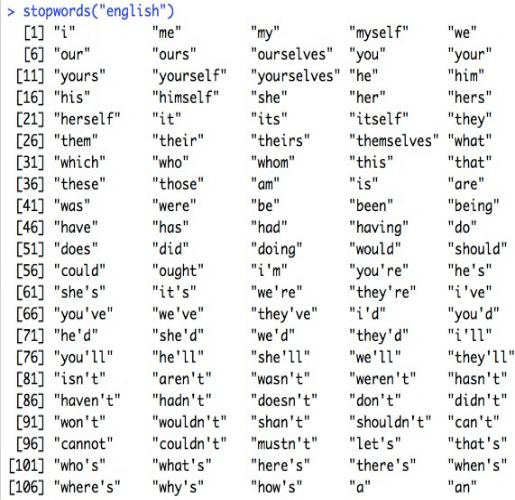
\includegraphics[height=2.5in]{stopwords}
		\caption[Stop words]{Stop words.}
		\label{fig:stopwords}
	\end{figure}


	\subsection{Stemming}
	\begin{bulletedlist}
		\item The idea of reducing different forms of a word to a core root.
		\item Words that are derived from one another can be mapped to a central word or symbol, especially if they have the same
core meaning.
		\item Used for dimensionality reduction.
		\item Word stem may not be present in dictionary, it does not cross check to ensure the new word is valid.
		\item and may not make sense in the sentence structure.  It just reduces the word to the stem without additional validation or checks.
		\item ``cook,'' ``cooking,'' and ``cooked'' all are reduced to same stem of ``cook.''
	\end{bulletedlist}

	\begin{figure}[h]
		\centering
		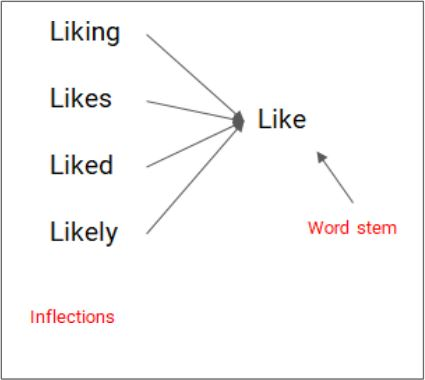
\includegraphics[height=1.5in]{wordstemming}
		\caption[Word stemming]{Word stemming.}
		\label{fig:wordstemming}
	\end{figure}


	\subsection{Lemmatization}
	\begin{bulletedlist}
		\item Lemmatization involves resolving words to their dictionary form.  A lemma of a word is its dictionary or canonical form.
		\item Lemmatization returns an actual word of the language, it is used where it is vital to get valid words.
		\item Examples:
		\begin{bulletedlist}
			\item walking $\rightarrow$ walk (core-word extraction)
			\item was $\rightarrow$ be (tense conversion to present tense)
			\item mice $\rightarrow$ mouse (plural to singular)
		\end{bulletedlist}
	\end{bulletedlist}

    \begin{table}[h]
        \centering
        \caption[stemming and lemmatization comparison]{Stemming and lemmatization comparison.}
        \label{tab:stemmingandlemma}
        \begin{tabular}{|c|c|c|} \hline
			\tablecolumnheadervlinesone{Word} 	& \tablecolumnheadervlinestwo{Stem}   & \tablecolumnheadervlinestwo{Lemma}\\ \hline
			Studies						        & Studi                               & Study \\ \hline
		\end{tabular}
	\end{table}



	\section{Statistical NLP}

    \begin{table}[h]
        \centering
        \caption[Statistical NLP]{Statistical natural language processing.}
        \label{tab:statisticalnlp}
        \begin{tabular}{|c|l|p{2in}|p{2in}|} \hline
			\tablecolumnheadervlinesone{No.} 	& \tablecolumnheadervlinestwo{Topic}   & \tablecolumnheadervlinestwo{Scope}   & \tablecolumnheadervlinestwo{Objective}\\ \hline
			1	& Bag of words	& Creating features using Bag of words, Countvectorizer	& Understand feature creation using Bag-Of-Words \\ \hline
			2	& Tf-IDF Model	& Term frequency, idf	& Understand difference between count-vectorizer and tf-idf vectorizer \\ \hline
			3	& Text classification using	ML	& How to use ML algorithm to do text classification		& Understand use cases of text classification \\ \hline
			4	& VADER Sentiment Analysis	& sentiment Analysis with VADER	& Brief idea on sentiment analysis \\ \hline
		\end{tabular}
	\end{table}

	\begin{figure}[h]
		\centering
		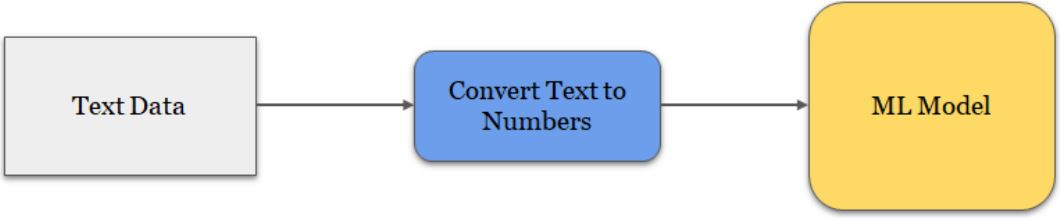
\includegraphics[width=4in]{posttextprocessing}
		\caption[Post text preprocessing]{Post text preprocessing.}
		\label{fig:posttextprocessing}
	\end{figure}

	\section{Word Representations}
	\begin{bulletedlist}
		\item Sparse
		\begin{bulletedlist}
			\item Term-document matrix or Document - Term matrix
			\begin{bulletedlist}
				\item Given a fixed vocabulary, we count the number of times each word occurs in a document for all documents. This matrix is the term - document matrix.
				\item We count the number of times a each word pair occurs in the document for a given vocabulary, resulting matrix is the term -term matrix.
			\end{bulletedlist}
			\item TF-IDF
		\end{bulletedlist}
	\end{bulletedlist}

	\section{Vectorization}
	\begin{bulletedlist}
		\item Tf-Idf vectors
		\begin{bulletedlist}
			\item Tf-idf is similar to term -document matrix with each word occurrence count divided by inverse document matrix.
		\end{bulletedlist}
		\item One-hot encoding of words.
		\item Above representations of documents are sparse since most of the elements in the matrix will be zero.
		\item These representations do not take into account individual word relationships.
	\end{bulletedlist}

	\section{Bag of Words}

	\begin{bulletedlist}
		\item Feature extraction approach in NLP.
		\item In this model, a text (such as a sentence or a document) is represented as the bag of its words, disregarding grammar and even word order but keeping multiplicity.
		\item We use the tokenized words for each observation and find out the frequency of each token.
		\item We define the vocabulary of corpus as all the unique words in the corpus above and below some certain threshold of frequency.
		\item Each sentence or document is defined by a vector of same dimension as vocabulary containing the frequency of each word of the vocabulary in the sentence.
		\item The bag-of-words model is commonly used in methods of document classification where the (frequency of) occurrence of each word is used as a feature for training a classifier.
	\end{bulletedlist}

	\begin{figure}[h]
		\centering
		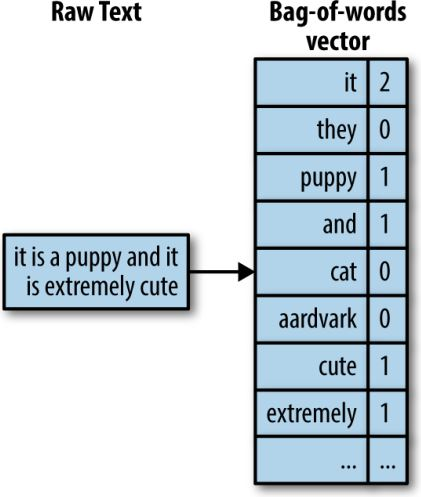
\includegraphics[height=2.25in]{bagofwords}
		\caption[Bag of words]{Bag of words.}
		\label{fig:bagofwords}
	\end{figure}


	\section{Tf-idf Vector}

	\begin{bulletedlist}
		\item TF-IDF (term frequency times inverse document frequency) is a scheme to weight individual tokens.
		\item One of the advantage of TF-IDF is reduce the impact of tokens that occur very frequently, hence offering little to none in terms of information.
	\end{bulletedlist}

	\begin{equation}
		TF = \frac{\textrm{frequency of a word in a document}}{\textrm{total number of words in the document}}
	\end{equation}


TF captures how important a word is to the document (without looking at the other documents in the data set).


Example: He is a good boy.  She is also good.
    \begin{table}[h]
        \centering
        \caption[Statistical NLP]{Statistical natural language processing.}
        \label{tab:stemmingandlemma}
        \begin{tabular}{|l|c|} \hline
        	\tabletitle{2}{Document 1} \\ \hline
			\tablecolumnheadervlinesone{Word} 	& \tablecolumnheadervlinestwo{Count}  \\ \hline
			he				& 1 \\ \hline
			is				& 2 \\ \hline
			a				& 1 \\ \hline
			good			& 2 \\ \hline
			boy				& 1 \\ \hline
			she				& 1 \\ \hline
			also			& 1 \\ \hline
			\textbf{total}	& \textbf{9} \\ \hline
		\end{tabular}
	\end{table}
	\begin{eqnarray}
		TF(he, doc1)  	& = 1/9  	& = 0.11	\\
		TF(good, doc1)	& = 2/9		& = 0.22
	\end{eqnarray}

Example 2: Radhika is a good person.
    \begin{table}[h]
        \centering
        \caption[Statistical NLP]{Statistical natural language processing.}
        \label{tab:stemmingandlemma}
        \begin{tabular}{|l|c|} \hline
        	\tabletitle{2}{Document 1} \\ \hline
			\tablecolumnheadervlinesone{Word} 	& \tablecolumnheadervlinestwo{Count}  \\ \hline
			Radhika		& 1 \\ \hline
			is			& 2 \\ \hline
			a			& 1 \\ \hline
			good		& 2 \\ \hline
			person		& 1 \\ \hline
			\textbf{total}	& \textbf{5} \\ \hline
		\end{tabular}
	\end{table}
	\begin{eqnarray}
		TF(he, doc1)  	& = 0/5  	& = 0	\\
		TF(good, doc1)	& = 1/5		& = 0.2
	\end{eqnarray}

	\begin{equation}
		IDF = \log\left(\frac{\textrm{number of documents}}{\textrm{number of documents word is in}}\right)
	\end{equation}

IDF tells us if a word (feature) can be used to distinguish documents. If a word appears in majority of the documents then IDF will be close to `0' i.e.\ give low weight to that feature.

	\begin{eqnarray}
		TF-IDF(he, doc1)  	& = 0.11*0.301  	& = 0.03311	\\
		TF-IDF(good, doc1)	& = 0.22*0			& = 0 \\
		TF-IDF(good, doc2)	& = 0*0.301			& = 0 \\
		TF-IDF(good, doc2)	& = 0.2*0			& = 0
	\end{eqnarray}

    \begin{table}[h]
        \centering
        \caption[TF-IDF example]{TF-IDF example.}
        \label{tab:stemmingandlemma}
        \begin{tabular}{|l|c|c|c|c|c|c|c|c|c|} \hline
			 & \tablecolumnheadervlinestwo{a} & \tablecolumnheadervlinestwo{also} & \tablecolumnheadervlinestwo{boy} & \tablecolumnheadervlinestwo{good} & \tablecolumnheadervlinestwo{he} & \tablecolumnheadervlinestwo{is} & \tablecolumnheadervlinestwo{person} & \tablecolumnheadervlinestwo{she} & \tablecolumnheadervlinestwo{Radhika} \\ \hline
			Index      & 0 & 1 & 2 & 3 & 4       & 5 & 6 & 7 & 8 \\ \hline
			Document 1 &   &   &   & 0 & 0.03311 &   &   &   &   \\ \hline
			Document 2 &   &   &   & 0 & 0       &   &   &   &   \\ \hline
		\end{tabular}
	\end{table}

	\section{N-gram}
	\begin{bulletedlist}
		\item It's a sequence of N-words.
		\item Bi-gram is a special case of N-grams where we consider only the sequence of two words.
		\item In N-gram models we calculate the probability of Nth words give the sequence of N-1 words. We do this by calculating the relative frequency of the sequence occurring in the text corpus.
	\end{bulletedlist}

	\begin{figure}[h]
		\centering
		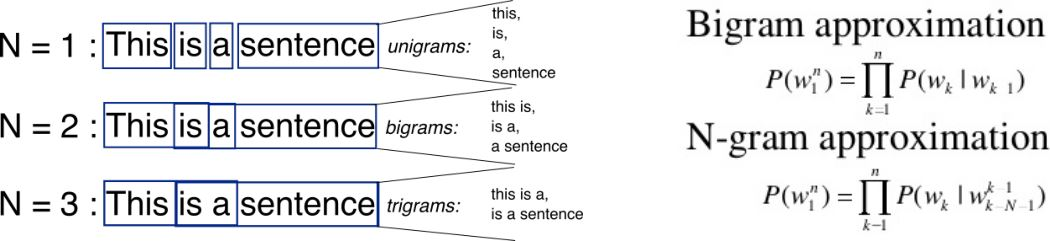
\includegraphics[height=1.25in]{ngram}
		\caption[N-gram]{N-gram.}
		\label{fig:ngram}
	\end{figure}

	\section{Text classifications using ML}
We can assign a category to different forms of text i.e. Articles, news, paragraphs, books, web pages etc.  Text classification has applications like spam filtering, sentiment analysis, document classification, text based analysis in marketing and product management.

	\section{Sentiment Analysis}
	\begin{bulletedlist}
		\item It's the content based subjective information retrieval obtained from monitoring online conversations.
		\item Used extensively to get overall end user feedback.
		\item Used for making text classification based automated mailing applications.
		\item Used for gaining insights on areas of improvement in product management.
	\end{bulletedlist}

	\section{VADER}
	\begin{bulletedlist}
		\item VADER (Valence Aware Dictionary and sEntiment Reasoner) is a lexicon and rule-based sentiment analysis tool that is specifically attuned to sentiments expressed in social media.
		\item VADER uses a combination of sentiment lexicon which is a list of lexical features (e.g., words) which are generally labelled according to their semantic orientation as either positive or negative.
		\item Like VADER sentiment analysis can be also be done using - NLTK, TextBlob.
	\end{bulletedlist}

	\section{Sentiment Analysis-Example}
	\begin{bulletedlist}
		\item Sentiment analysis - positive or negative
		\begin{bulletedlist}
			\item ``This is a ridiculously priced toothbrush.  Seriously, no way to get around it. It is absurdly priced and I'm almost embarrassed to be admitting that I bought it.  With that said... Wow, this thing is amazing.''
			\item ``These pens make me feel so feminine and desirable. I can barely keep the men away when I'm holding one of these in my dainty hand.  My husband has started to take fencing lessons just to keep the men away.''
		\end{bulletedlist}
	\end{bulletedlist}
